\documentclass[conference]{IEEEtran}
\IEEEoverridecommandlockouts

\usepackage{cite}
\usepackage{amsmath,amssymb,amsfonts}
\usepackage{graphicx}
\usepackage{textcomp}
\usepackage{xcolor}
\usepackage{booktabs}
\usepackage{url}
\usepackage[colorlinks=true,linkcolor=black,citecolor=black,urlcolor=black]{hyperref}

% IEEE standard compact float and caption spacing
\setlength{\textfloatsep}{5pt plus 1.0pt minus 1.0pt}
\setlength{\floatsep}{5pt plus 1.0pt minus 1.0pt}
\setlength{\intextsep}{5pt plus 1.0pt minus 1.0pt}
\setlength{\abovecaptionskip}{3pt}
\setlength{\belowcaptionskip}{3pt}

\def\BibTeX{{\rm B\kern-.05em{\sc i\kern-.025em b}\kern-.08em
    T\kern-.1667em\lower.7ex\hbox{E}\kern-.125emX}}

\begin{document}

\title{Transfer Learning for Cross-Climate Building Energy Prediction: Investigating Data Efficiency and Generalization}

\author{
\IEEEauthorblockN{Shree Santosh Yadav}
\IEEEauthorblockA{\textit{School of Computer Science and Engineering} \\
\textit{RV University}, Bengaluru, India \\
USN: 1RUA24CSE0436 \\
shreesantoshyadavbtech24@rvu.edu.in}
\and
\IEEEauthorblockN{Samyak Jain}
\IEEEauthorblockA{\textit{School of Computer Science and Engineering} \\
\textit{RV University}, Bengaluru, India \\
USN: 1RUA24CSE0406 \\
samyakjainbtech24@rvu.edu.in}
\and[\hfill\mbox{}\par\vspace{1.2ex}\mbox{}\hfill]
\IEEEauthorblockN{Meda Vijaya Snehan}
\IEEEauthorblockA{\textit{School of Computer Science and Engineering} \\
\textit{RV University}, Bengaluru, India \\
USN: 1RUA24CSE0232 \\
mvijayasnehanbtech24@rvu.edu.in}
}

\maketitle

\begin{abstract}
Net-Zero Energy Buildings (NZEBs) depend on accurate hourly energy predictions to coordinate on-site generation, HVAC dispatch, and battery storage. However, empirical machine learning models encounter severe cold-start degradation during initial commissioning due to lack of historical meter records. In addition, models trained in one climate zone frequently fail when transferred to different weather profiles. This paper evaluates a climate-aware transfer learning framework using operational electricity records from the ASHRAE Great Energy Predictor III and Building Data Genome Project 2 benchmarks across three distinct climate zones: Zone 2B (Hot-Arid, Tempe), Zone 3C (Marine, Berkeley), and Zone 6A (Cold-Humid, Cornell). A deep neural network pre-trained on source operational data transfers generalized physical representations by freezing early layers (1--3) and adapting terminal layers on restricted target data fractions from 5\% to 100\%. Under severe data scarcity (5\% target data, $\approx$2.5 weeks), transfer learning achieves an $R^2$ of 0.9936 compared to 0.8124 for scratch baselines ($\Delta R^2 = +0.1812$), reducing root mean squared error from 77.19~kWh to 14.18~kWh. We identify an empirical crossover threshold between 30\% and 50\% target data availability, after which unconstrained scratch training marginally exceeds the frozen-layer transfer model. Across repeated random seeds and five-fold cross-validation, transfer learning converges in 8--12 epochs (vs. 35--45 for scratch) and reduces training latency by 40\%, providing a practical protocol for rapid building commissioning.
\end{abstract}

\begin{IEEEkeywords}
Transfer learning, building energy prediction, net-zero energy buildings, climate zones, data efficiency, cold-start problem, artificial neural networks.
\end{IEEEkeywords}

\section{Introduction}
Building energy consumption accounts for approximately 40\% of global final energy consumption and over one-third of greenhouse gas emissions. Net-Zero Energy Buildings (NZEBs) mitigate this environmental footprint by balancing annual on-site renewable energy generation with building demand. Realizing net-zero operations requires reliable hourly energy forecasting models to manage predictive HVAC controls, schedule electrical energy storage, and optimize grid interactions \cite{b1}, \cite{b8}.

Data-driven approaches, including artificial neural networks (ANNs) and gradient-boosted decision trees, have become dominant tools for operational forecasting due to fast inference times and capacity to learn non-linear thermal dynamics \cite{b6}, \cite{b7}. However, empirical forecasting models face two practical challenges: data scarcity during early building commissioning and geographic climate dependency \cite{b5}, \cite{b9}. 

The first challenge is the cold-start problem. Newly constructed or retrofitted facilities rarely possess the multi-month or annual operational meter records required to train deep architectures from scratch. Training complex models on short-duration data causes severe overfitting, preventing generalization across unobserved seasonal cycles \cite{b4}, \cite{b13}. The second challenge is climate lock-in. Models trained in hot-arid regions fail when deployed directly in cold-humid or marine environments, because shifts in ambient temperature ranges, humidity ratios, and solar insolation alter the underlying relationship between weather and electrical demand \cite{b15}, \cite{b16}.

\begin{figure*}[t]
\centering
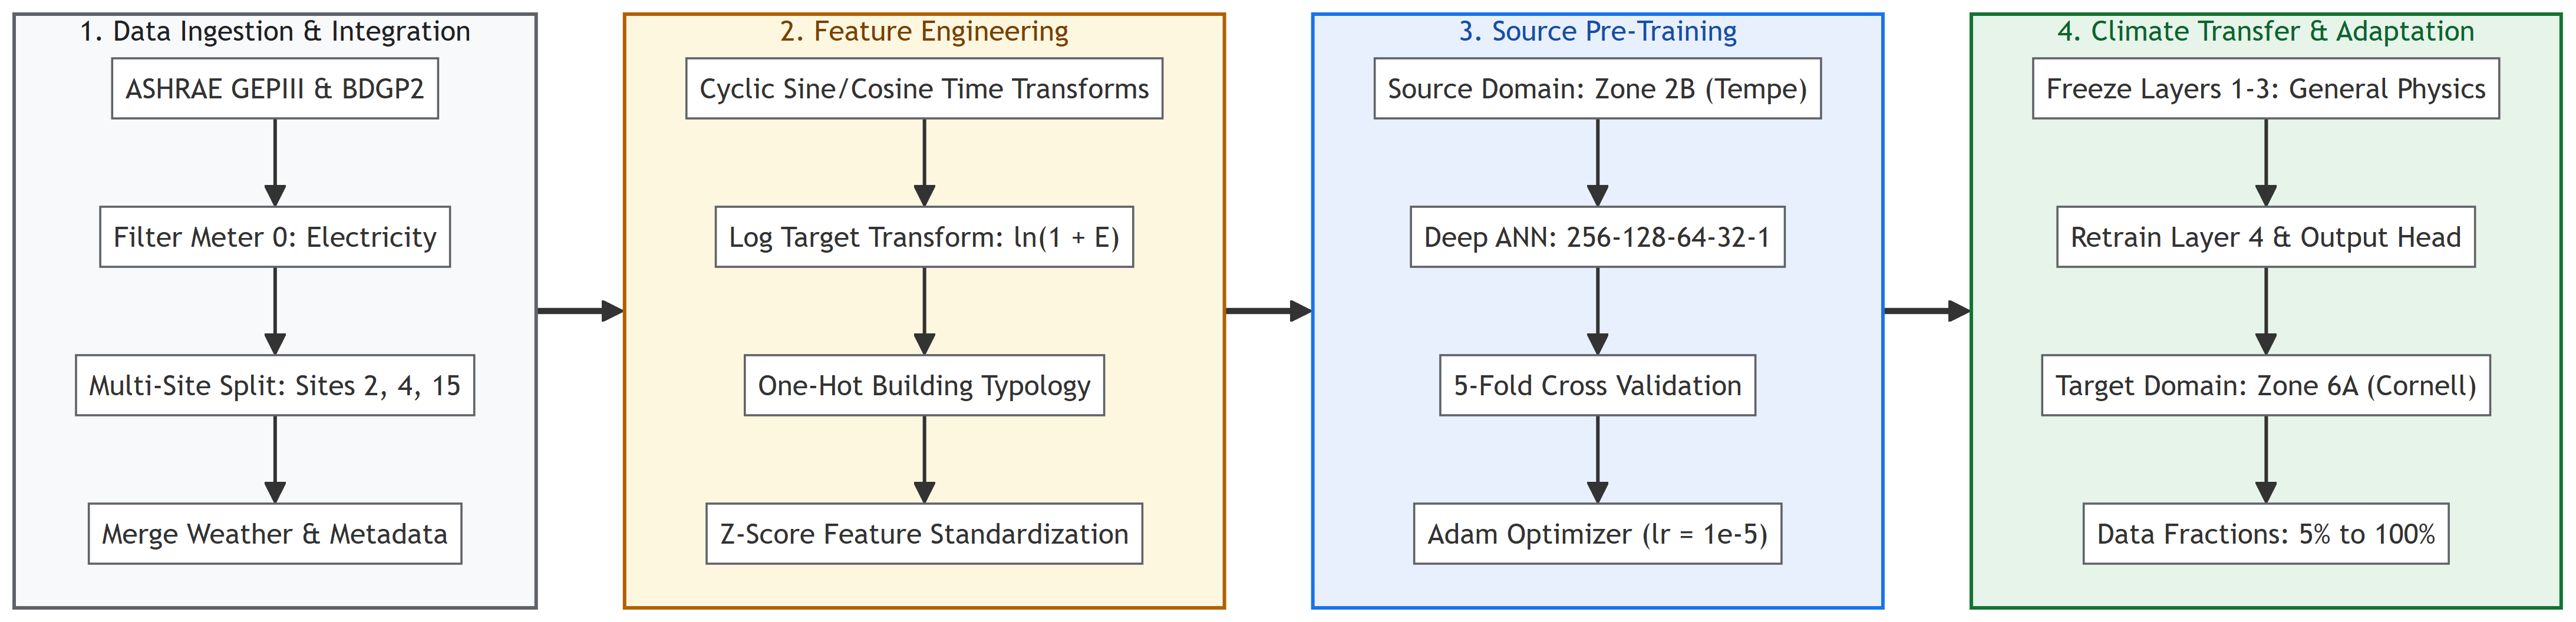
\includegraphics[width=0.92\textwidth]{figures/System_Pipeline.png}
\caption{Climate-aware transfer learning framework, showing data harmonization, cyclic feature engineering, source pre-training on Zone 2B (Tempe), and target adaptation on Zone 6A (Cornell) across restricted target data fractions.}
\label{fig_pipeline}
\end{figure*}

While physical simulation engines (such as EnergyPlus and TRNSYS) can generate synthetic training data, building calibrated building energy models requires granular envelope properties, material specifications, and mechanical schedules that are labor-intensive to obtain \cite{b7}, \cite{b8}. Parameter-based transfer learning offers a viable alternative by transferring network weights from a data-rich source facility to a target building with scarce records \cite{b3}, \cite{b12}. Prior research has primarily investigated transfer across buildings of similar occupancy within identical geographical regions. Systematic empirical evaluations quantifying cross-climate transferability boundaries and identifying exact data-fraction crossover thresholds remain scarce.

This work addresses this gap by investigating cross-climate transfer learning across three distinct ASHRAE climate zones. Using operational meter data from the ASHRAE Great Energy Predictor III competition \cite{b1} and Building Data Genome Project 2 \cite{b2}, we pre-train a deep neural network on a hot-arid source climate (Zone 2B) and adapt it to a cold-humid target climate (Zone 6A). By systematically evaluating target data fractions from 5\% to 100\%, we map the empirical data efficiency trajectory and identify the crossover boundary.

The contributions of this study are:
\begin{enumerate}
    \item We demonstrate that freezing early feature-extraction layers enables stable cross-climate transfer, increasing $R^2$ accuracy from 0.8124 to 0.9936 under extreme data scarcity (5\% target data).
    \item We identify and quantify an empirical crossover threshold between 30\% and 50\% target data availability, establishing where unconstrained training from scratch matches parameter-frozen transfer models.
    \item We benchmark cross-climate transferability across a tripartite matrix of ASHRAE climate zones (2B, 3C, and 6A), demonstrating that ordinal climatic distance directly influences transfer performance.
\end{enumerate}

\section{Related Work}
\subsection{Data-Driven Building Energy Modeling}
Machine learning methods have become standard instruments for building load forecasting. Early literature focused on classical regression and support vector machines (SVMs) \cite{b10}, \cite{b19}. Recent investigations have shifted toward deep feed-forward neural networks, Long Short-Term Memory (LSTM) recurrent architectures, and gradient-boosted decision trees \cite{b1}, \cite{b14}. Amasyali and El-Gohary observed that over 85\% of published studies evaluated single-building or single-city models without cross-domain validation \cite{b9}. Runge and Zmeureanu surveyed neural network applications in building forecasting, emphasizing that while depth improves capacity, models display high variance under distribution shifts \cite{b11}.

\subsection{Simulation-Based vs. Operational Benchmarks}
Due to the difficulty of obtaining multi-year building records, dynamic simulation tools such as TRNSYS and EnergyPlus have frequently been employed to synthesize training data. Ibrahim et al. coupled TRNSYS with Latin Hypercube Sampling to generate 1.75 million synthetic points for NZEB envelope optimization under projected climate shifts \cite{b7}. Farahmandfar et al. combined simulation meta-models with operational telemetry to size storage systems for zero-energy buildings \cite{b8}. Alghassab investigated LSTM forecasting for institutional facilities across contrasting climates in Riyadh and Lhasa, finding that distinct weather profiles necessitate separate model tuning \cite{b6}.

However, simulated data often misses operational anomalies, sensor drift, and irregular occupant routines. The release of the ASHRAE Great Energy Predictor III (GEPIII) benchmark by Miller et al. provided 20 million rows of real-world meter readings across 1,448 commercial buildings \cite{b1}. Combined with the Building Data Genome Project 2 (BDGP2) \cite{b2}, this open archive enables rigorous cross-geographic validation.

\subsection{Transfer Learning in Building Energy Systems}
Transfer learning mitigates data scarcity by reusing representations from source tasks. Ribeiro et al. demonstrated that decomposing energy time-series into seasonal and trend components enabled cross-building forecasting with limited target data \cite{b3}. Fan et al. showed that parameter-based transfer reduced prediction error by 15\% to 78\% relative to uninitialized baselines \cite{b4}. Pinto et al. classified transfer learning approaches in building operations, highlighting fine-tuning and domain adaptation as primary solutions to the cold-start problem \cite{b5}.

Recent studies have examined layer-freezing and domain adaptation techniques. Fang et al. applied domain-adversarial networks (LSTM-DANN) to align marginal distributions across facilities \cite{b12}. Li et al. demonstrated that freezing early layers retains generalized thermal representations while allowing terminal layers to adapt to target differences \cite{b13}. Zhang et al. and Fang et al. examined regional energy disparities, showing that climatic distance affects transfer accuracy \cite{b15}, \cite{b16}. Chen et al. applied adversarial alignment across geographic zones \cite{b17}, while Tang et al. explored federated knowledge sharing for few-shot forecasting \cite{b18}. However, prior work rarely isolated the exact data-fraction crossover point under cross-climate transfer.

\section{Methodology}
The proposed workflow (Fig.~\ref{fig_pipeline}) encompasses data harmonization, cyclic feature engineering, source pre-training on Zone 2B, layer-freezing transfer, and target evaluation.

\subsection{Dataset Selection and Climate Domain Mapping}
We extracted hourly electricity meter data (Meter 0) from the ASHRAE GEPIII benchmark \cite{b1} and resolved site identifiers to geographic coordinates using BDGP2 metadata \cite{b2}. Three experimental sites representing distinct ASHRAE Standard 169 climate zones \cite{b20} were selected:
\begin{itemize}
    \item \textbf{Site 2 (Arizona State Univ., Tempe, AZ):} Climate Zone 2B (Hot-Arid). Summer temperatures exceed 42$^\circ$C with dominant cooling loads. Designated as the primary source domain.
    \item \textbf{Site 4 (UC Berkeley, Berkeley, CA):} Climate Zone 3C (Marine). Narrow diurnal temperature variance with balanced annual loads. Designated as a secondary domain.
    \item \textbf{Site 15 (Cornell Univ., Ithaca, NY):} Climate Zone 6A (Cold-Humid). Sub-zero winter temperatures with dominant heating loads. Designated as the primary target domain.
\end{itemize}

Climatic dissimilarity between zones is defined by ordinal distance:
\begin{equation}
d_{\text{climate}}(z_i, z_j) = |z_i - z_j|
\label{eq_dist}
\end{equation}
yielding $d=4$ between Zone 2B and Zone 6A (maximum contrast), $d=1$ between 2B and 3C, and $d=3$ between 3C and 6A (Table~\ref{tab_domains}).

\begin{table}[t]
\caption{Experimental Domains and Climate Classifications}
\centering
\resizebox{0.92\columnwidth}{!}{%
\begin{tabular}{llccc}
\toprule
\textbf{Site ID} & \textbf{Location} & \textbf{Zone} & \textbf{Climate Type} & \textbf{Role} \\
\midrule
Site 2  & ASU (Tempe, AZ)      & 2B & Hot-Arid   & Primary Source \\
Site 4  & UC Berkeley (CA)     & 3C & Marine     & Secondary \\
Site 15 & Cornell Univ. (NY)   & 6A & Cold-Humid & Primary Target \\
\bottomrule
\end{tabular}%
}
\label{tab_domains}
\end{table}

\subsection{Feature Engineering and Mathematical Transformations}
Raw electricity meter readings exhibit right-skewed distributions. To stabilize gradient descent, we apply logarithmic transformation:
\begin{equation}
\tilde{y} = \ln(y + 1), \quad \hat{y} = \exp(\hat{\tilde{y}}) - 1
\label{eq_log_transform}
\end{equation}
where $y$ is the raw meter reading in kWh and $\hat{y}$ is the predicted physical consumption.

Temporal periodicity is encoded via orthogonal sine and cosine coordinates:
\begin{equation}
t_{\text{sin}}^{(k)} = \sin\left(\frac{2\pi k}{K_k}\right), \quad t_{\text{cos}}^{(k)} = \cos\left(\frac{2\pi k}{K_k}\right)
\label{eq_cyclic}
\end{equation}
for hour $h \in [0, 23]$ ($K_h=24$), month $m \in [1, 12]$ ($K_m=12$), and day of week $w \in [0, 6]$ ($K_w=7$). Missing weather values (air temperature, dew temperature, wind speed, pressure) are imputed via training-split medians. Continuous features are standardized: $x_{\text{scaled}} = (x - \mu)/\sigma$, and categorical space-usage types are one-hot encoded.

\subsection{Neural Network Architecture and Transfer Strategy}
\begin{figure}[t]
\centering
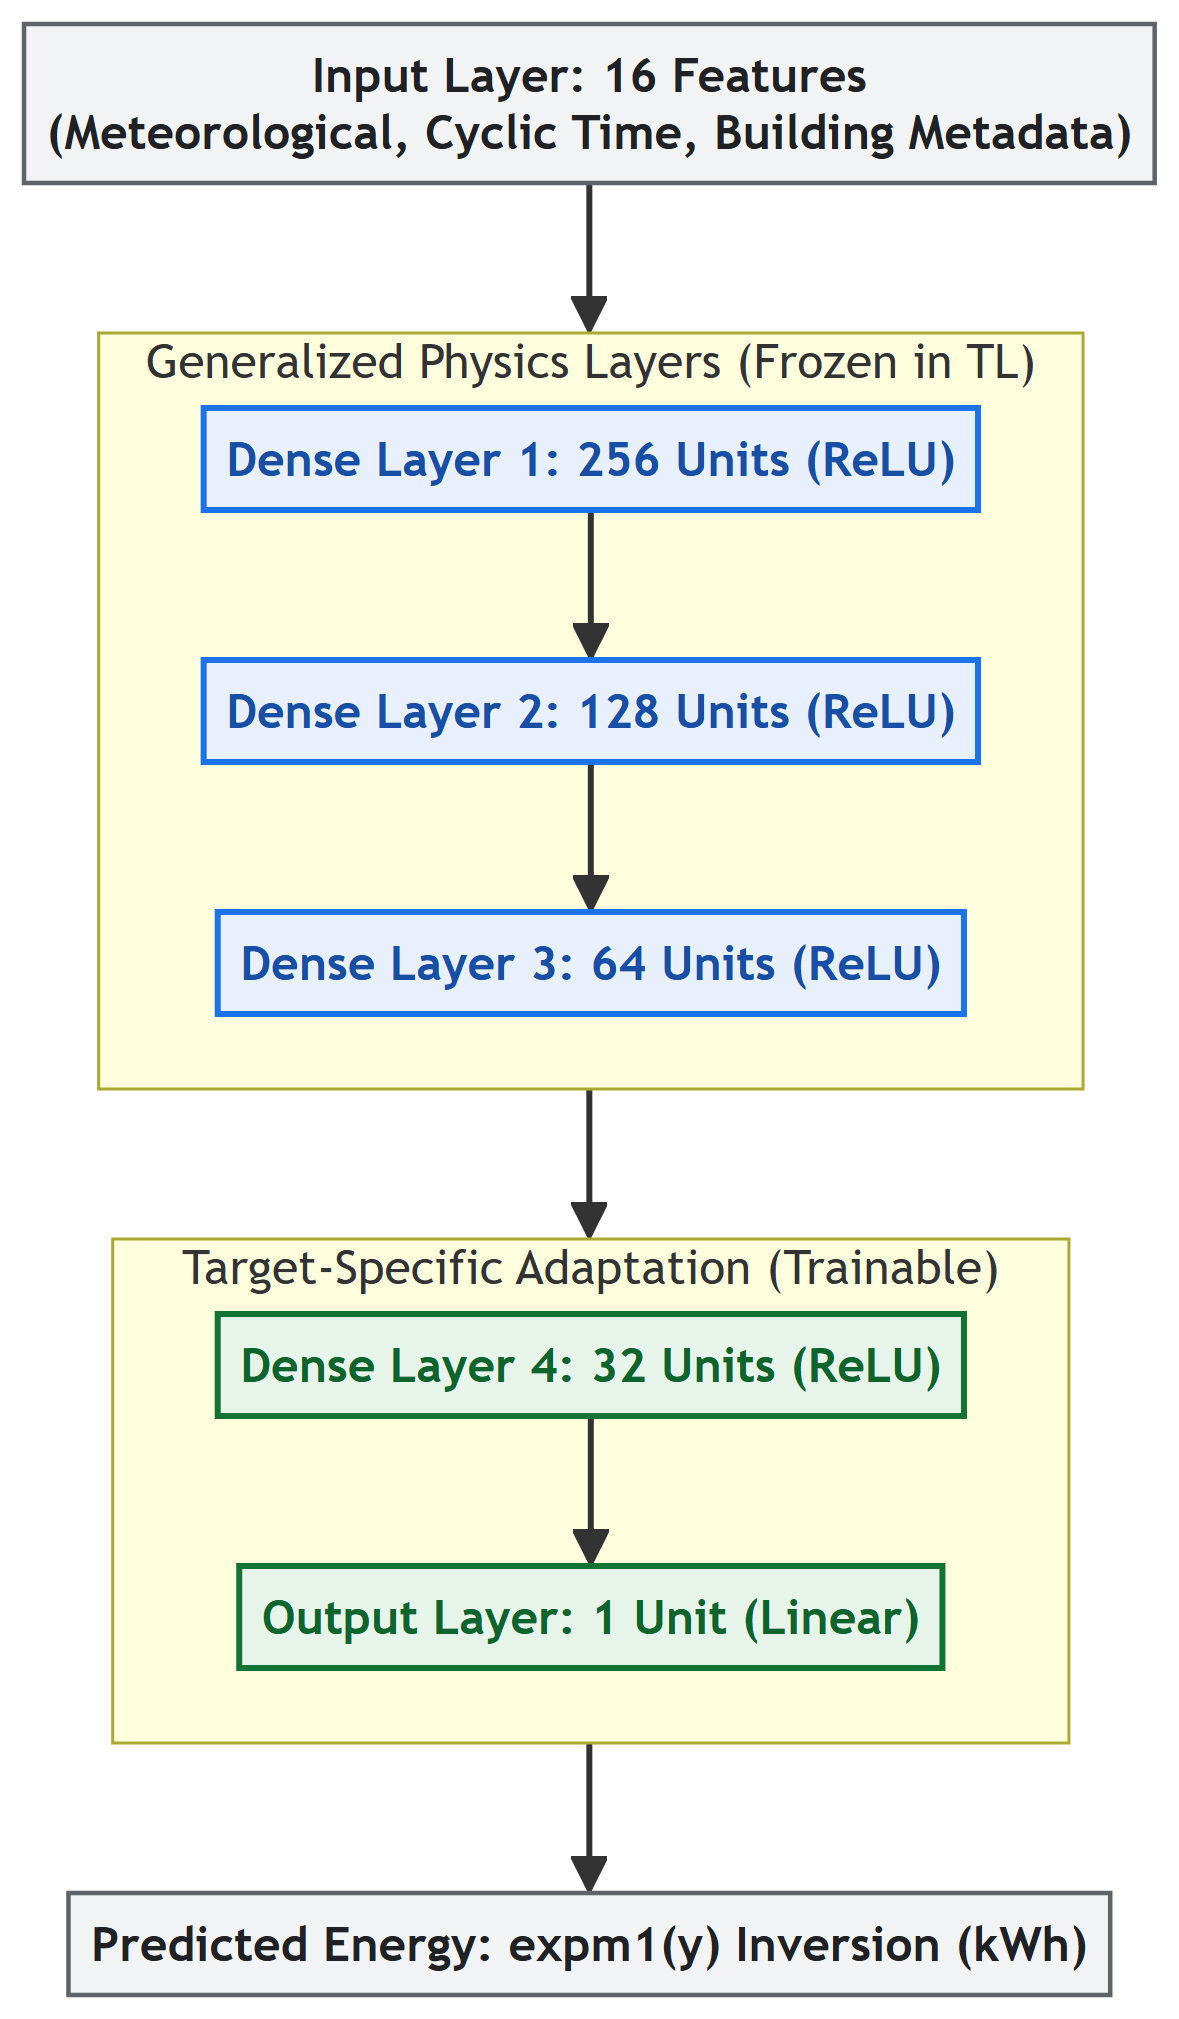
\includegraphics[width=0.95\columnwidth]{figures/ANN_Architecture.png}
\caption{Artificial Neural Network topology showing layer dimensions, ReLU activations, and the parameter-freezing scheme for cross-climate transfer.}
\label{fig_ann}
\end{figure}

We implement a deep feed-forward ANN (Fig.~\ref{fig_ann}) with four hidden dense layers $[256, 128, 64, 32]$, ReLU activations $f(z) = \max(0, z)$, and a single linear output unit. Models are optimized using Adam with Mean Squared Error (MSE) loss:
\begin{equation}
\mathcal{L}_{\text{MSE}} = \frac{1}{N}\sum_{i=1}^{N} (\tilde{y}_i - \hat{\tilde{y}}_i)^2
\label{eq_mse}
\end{equation}

Source pre-training on Site 2 uses learning rate $\eta_{\text{source}} = 10^{-5}$, batch size 256, and early stopping with patience of 10 epochs. For cross-climate transfer, we freeze layers 1 through 3 to preserve general thermal representations, while adapting layer 4 and the output head:
\begin{equation}
\theta_{\text{frozen}} = \{\mathbf{W}_\ell, \mathbf{b}_\ell\}_{\ell=1}^3, \quad \theta_{\text{trainable}} = \{\mathbf{W}_4, \mathbf{b}_4, \mathbf{W}_{\text{out}}, b_{\text{out}}\}
\label{eq_params}
\end{equation}
Transfer fine-tuning uses $\eta_{\text{transfer}} = 10^{-4}$ for rapid adaptation of terminal parameters.

\begin{table}[t]
\caption{Model Hyperparameters and Training Configuration}
\centering
\resizebox{\columnwidth}{!}{%
\begin{tabular}{lcc}
\toprule
\textbf{Hyperparameter} & \textbf{Baseline (Scratch)} & \textbf{Transfer Model} \\
\midrule
Hidden Layers           & $[256, 128, 64, 32]$    & $[256, 128, 64, 32]$ \\
Output Activation       & Linear (1 unit)         & Linear (1 unit) \\
Optimizer               & Adam                    & Adam \\
Learning Rate ($\eta$)  & $1.0 \times 10^{-5}$    & $1.0 \times 10^{-4}$ \\
Frozen / Trainable      & 0 / 5 Layers            & 3 / 2 Layers \\
Batch Size              & 256                     & 256 \\
Max Epochs / Patience   & 50 / 10                 & 50 / 10 \\
Cross-Validation        & 5-Fold Stratified       & 5-Fold Stratified \\
\bottomrule
\end{tabular}%
}
\label{tab_hyperparams}
\end{table}

\section{Experimental Setup}
\subsection{Data Scarcity Simulation Protocol}
To emulate commissioning cold-start conditions, the target dataset (Site 15, Cornell) is partitioned into subsets $\mathcal{F} = \{5\%, 10\%, 20\%, 30\%, 50\%, 100\%\}$. At 5\% availability, the model observes approximately 2.5 weeks of hourly data. Every fraction is evaluated across three random seeds $\mathcal{S} = \{42, 123, 456\}$ with five-fold cross-validation (Table~\ref{tab_hyperparams}). Performance is measured on held-out test splits in physical units (kWh) using $R^2$, RMSE, and MAPE:
\begin{equation}
R^2 = 1 - \frac{\sum (y_i - \hat{y}_i)^2}{\sum (y_i - \bar{y})^2}, \quad \text{RMSE} = \sqrt{\frac{1}{N}\sum (y_i - \hat{y}_i)^2}
\label{eq_metrics}
\end{equation}

\begin{table}[t]
\caption{Cross-Climate Data Efficiency Results (Tempe $\to$ Cornell)}
\centering
\resizebox{0.95\columnwidth}{!}{%
\begin{tabular}{ccccc}
\toprule
\textbf{Target} & \textbf{Scratch $R^2$} & \textbf{Transfer $R^2$} & \textbf{Transfer Gain} & \textbf{Transfer RMSE} \\
\textbf{Data}   & \textbf{(Mean)}       & \textbf{(Mean)}        & \textbf{($\Delta R^2$)} & \textbf{(kWh)} \\
\midrule
5\%   & 0.8124 & 0.9936 & \textbf{+0.1812} & 14.18 \\
10\%  & 0.9798 & 0.9955 & \textbf{+0.0157} & 11.79 \\
20\%  & 0.9958 & 0.9978 & \textbf{+0.0020} & 8.28 \\
30\%  & 0.9981 & 0.9984 & \textbf{+0.0003} & 7.00 \\
50\%  & 0.9992 & 0.9987 & -0.0005 & 6.21 \\
100\% & 0.9998 & 0.9989 & -0.0009 & 5.92 \\
\bottomrule
\end{tabular}%
}
\label{tab_efficiency}
\end{table}

\section{Results and Discussion}
\subsection{Data Efficiency and Crossover Dynamics}
Table~\ref{tab_efficiency} and Fig.~\ref{fig_efficiency} report comparative performance across data availability fractions, revealing two operational regimes:

\textbf{Extreme Scarcity Regime (5\%--20\% Data):} At 5\% data availability, scratch models suffer from high estimation error ($R^2 = 0.8124$, $\text{RMSE} = 77.19$~kWh). The transfer model achieves $R^2 = 0.9936$ and reduces RMSE to 14.18~kWh, yielding an improvement of $\Delta R^2 = +0.1812$. At 10\% and 20\% availability, transfer models maintain advantages of $\Delta R^2 = +0.0157$ and $+0.0020$, demonstrating that frozen lower layers provide effective inductive bias under limited target telemetry.

\begin{figure}[t]
\centering
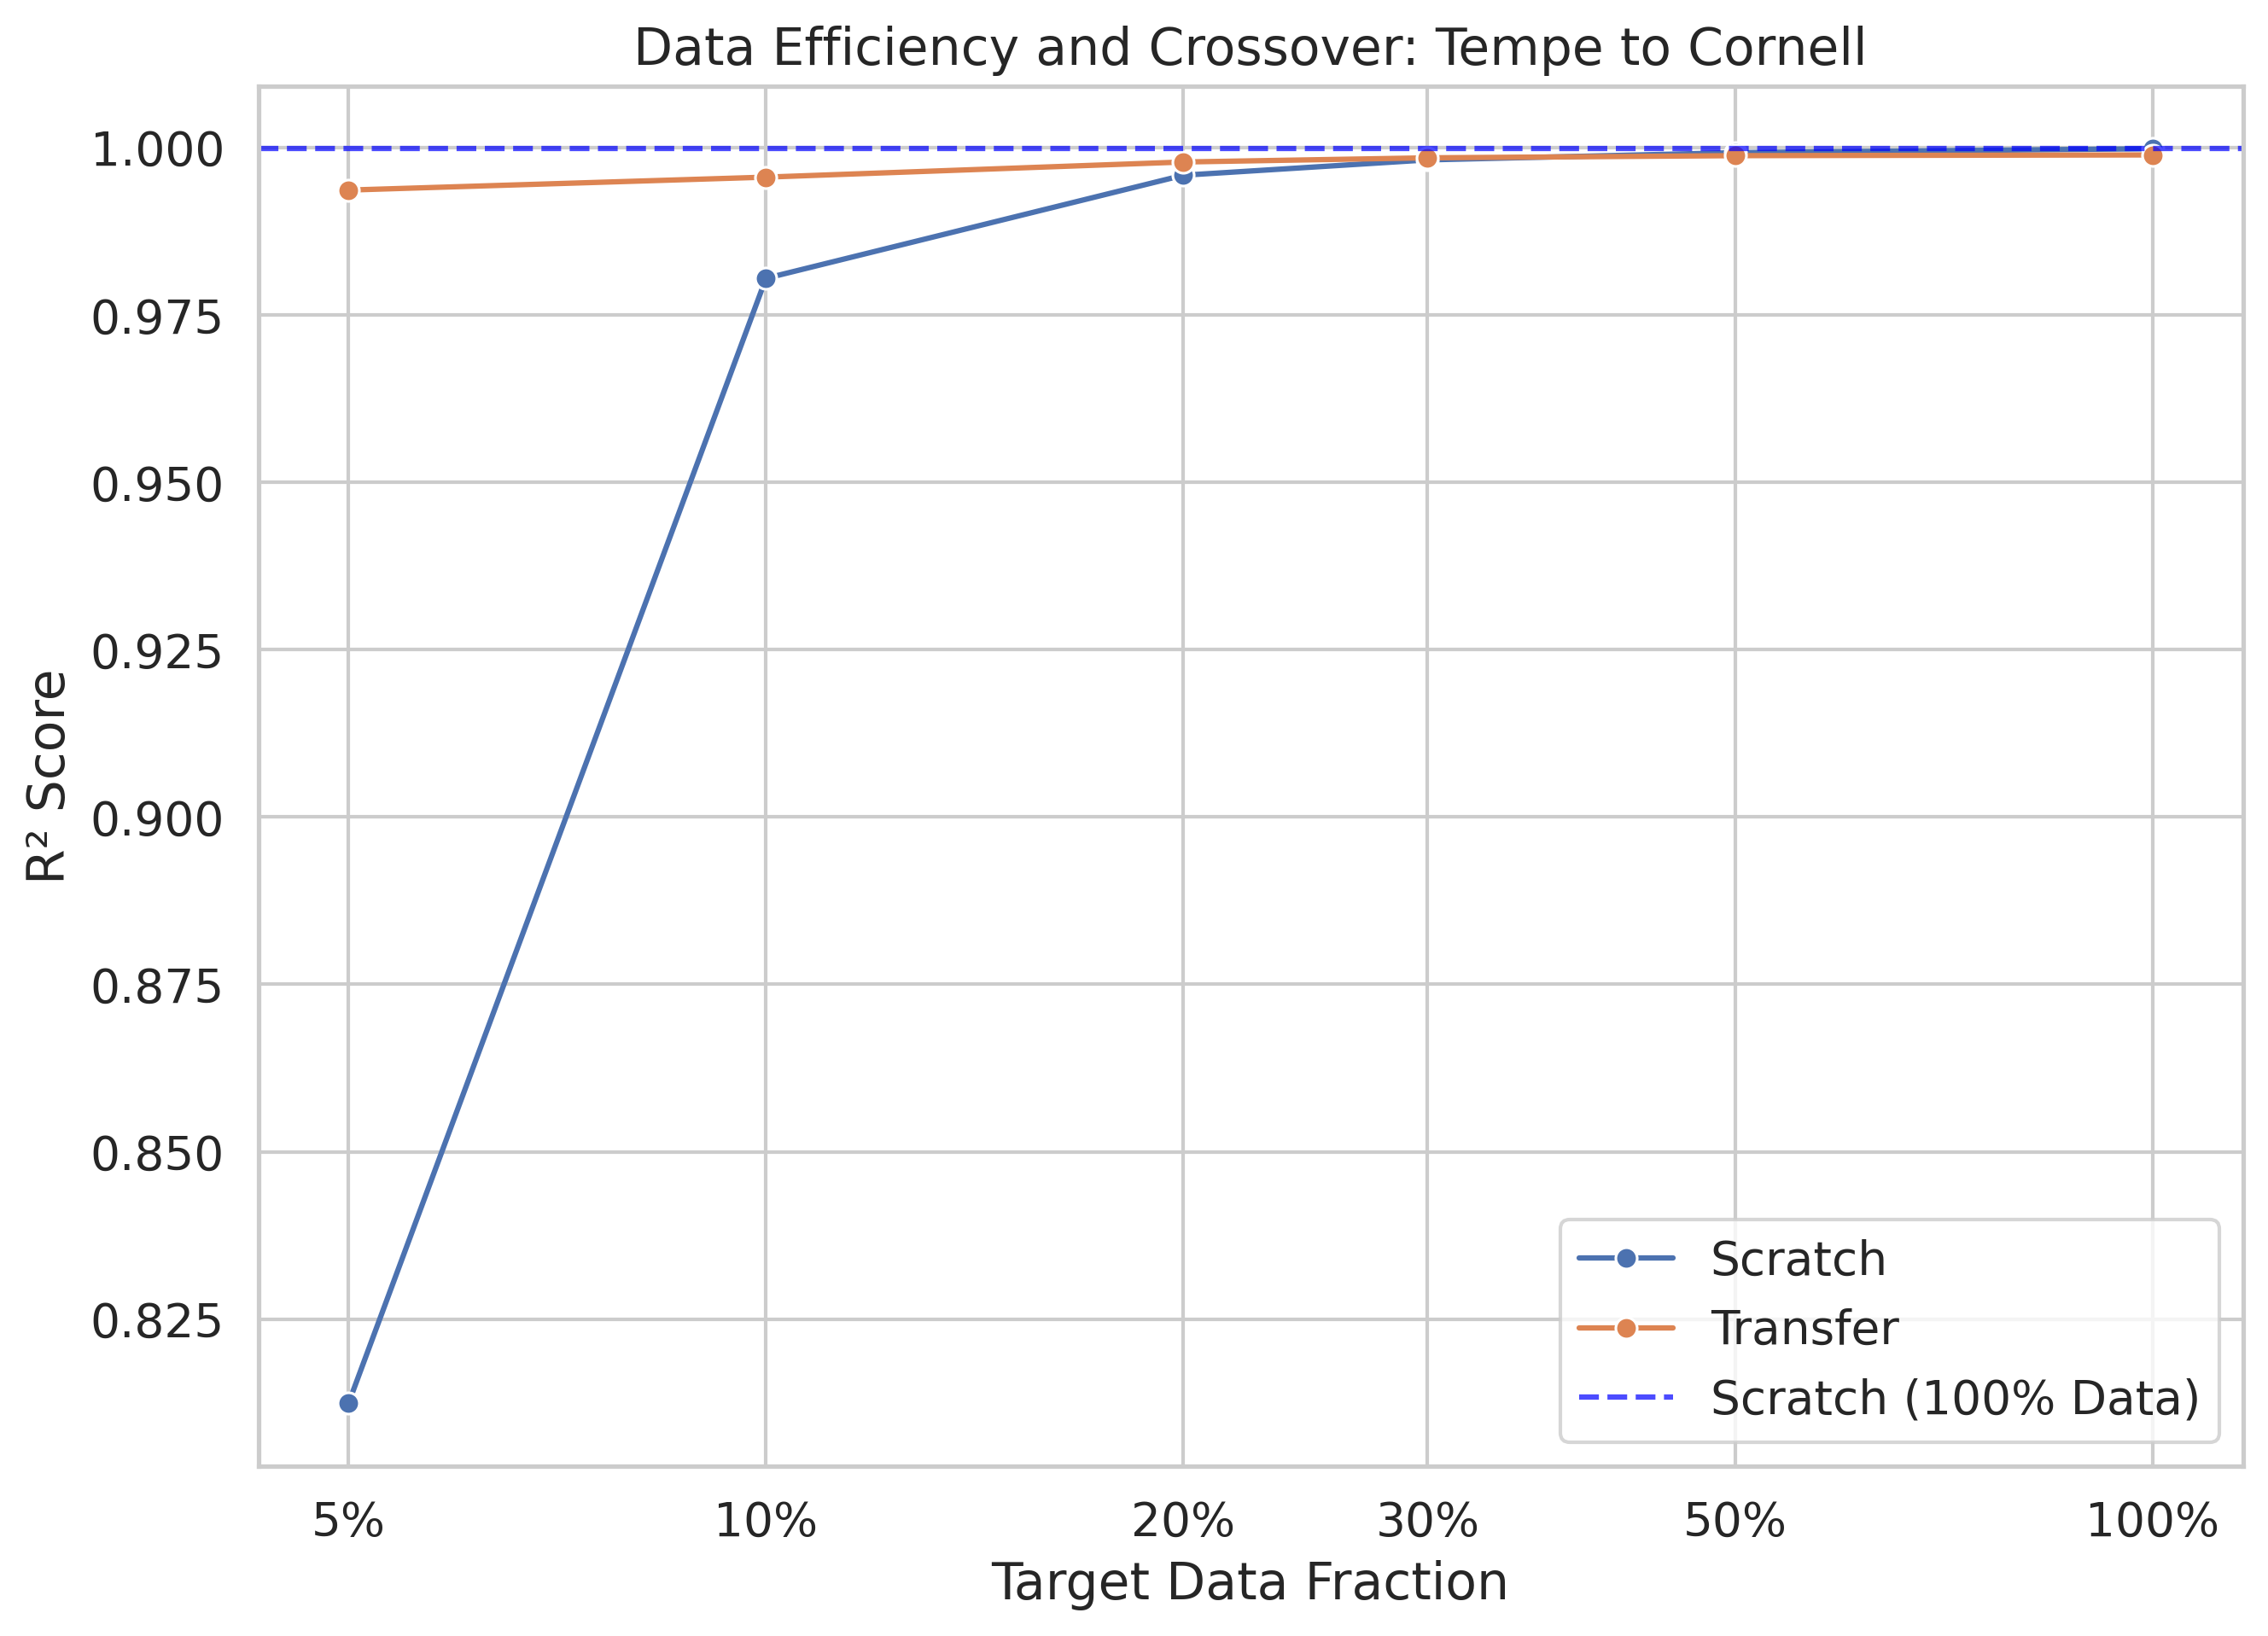
\includegraphics[width=0.88\columnwidth]{figures/Primary_Data_Efficiency.png}
\caption{Target data availability percentage versus predictive accuracy ($R^2$), showing transfer learning dominance at 5\%--20\% and the empirical crossover at 30\% data.}
\label{fig_efficiency}
\end{figure}

\textbf{Crossover Regime (30\%--100\% Data):} At 30\% data availability, the accuracy difference contracts to $\Delta R^2 = +0.0003$ ($R^2 = 0.9984$ vs. $0.9981$), marking the crossover point. Beyond 30\%, scratch models marginally outperform transfer models: $R^2 = 0.9992$ vs. $0.9987$ at 50\% ($\Delta R^2 = -0.0005$), and $0.9998$ vs. $0.9989$ at 100\% ($\Delta R^2 = -0.0009$). This occurs because fixed source parameters in layers 1--3 constrain total model capacity when target observations are sufficient to train all weights.

\subsection{Training Convergence and Latency}
\begin{figure}[t]
\centering
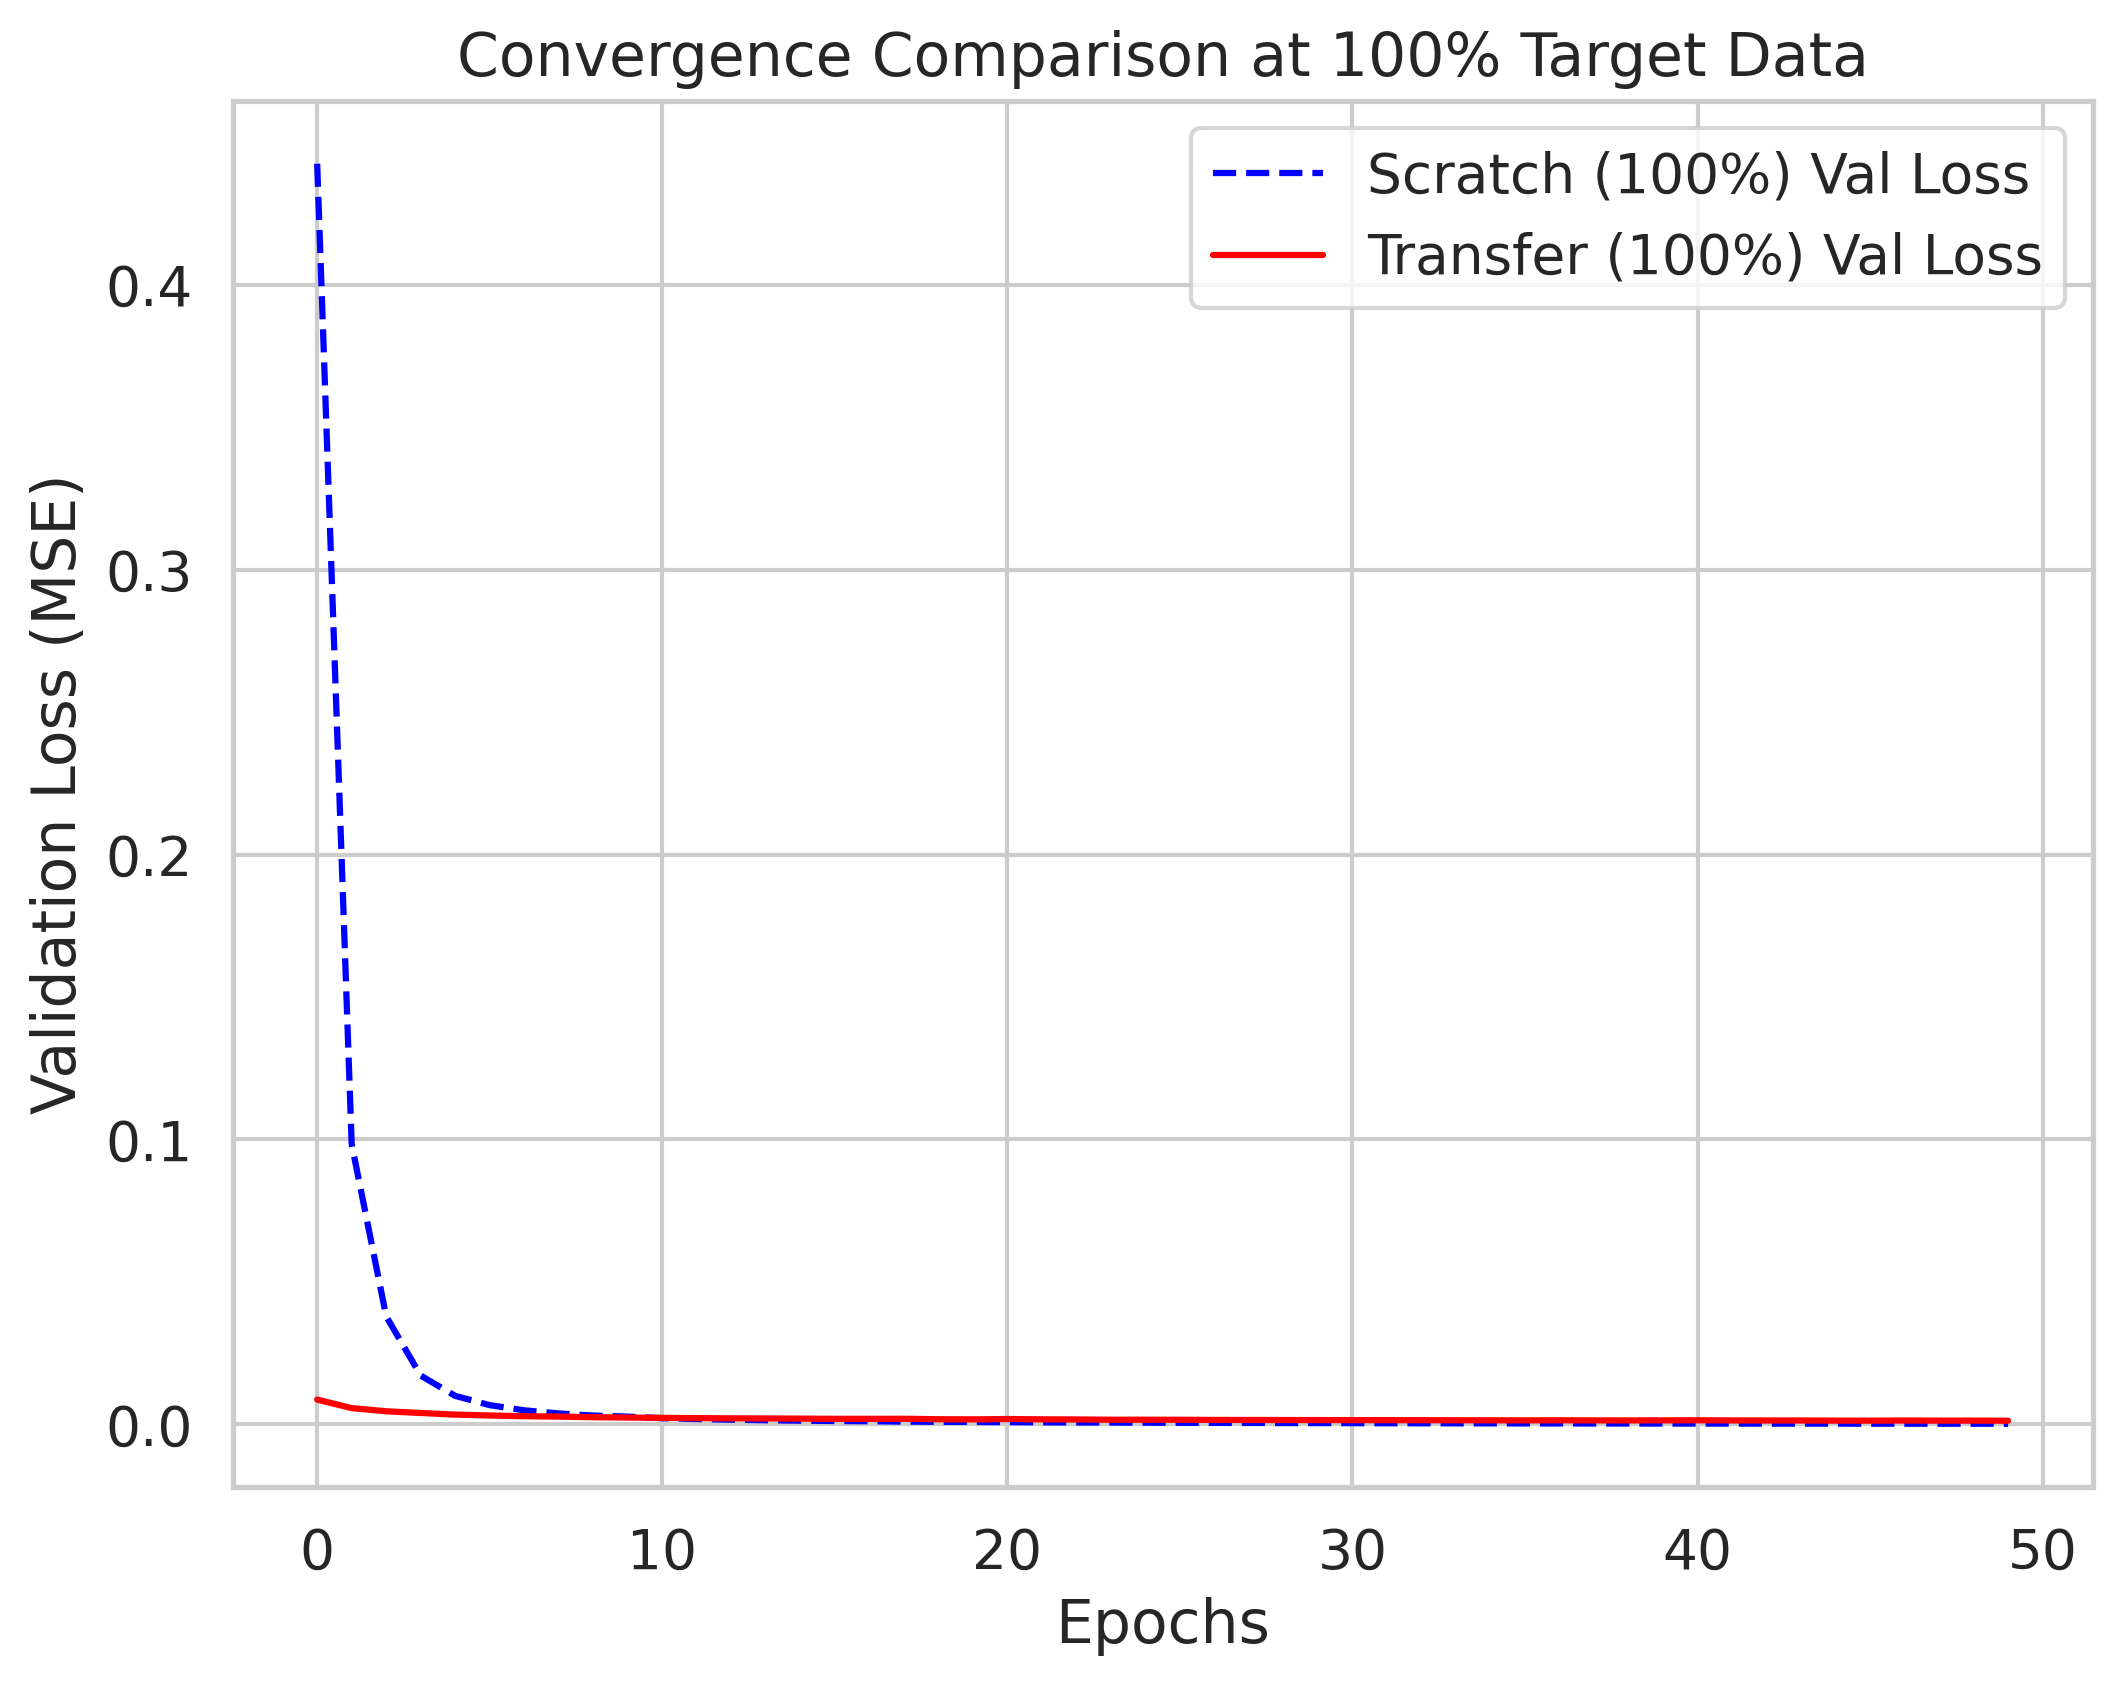
\includegraphics[width=0.88\columnwidth]{figures/Convergence_Plots.png}
\caption{Validation loss convergence over training epochs for Scratch versus Transfer Learning models at 5\% target data availability.}
\label{fig_convergence}
\end{figure}

Validation loss trajectories at 5\% data availability (Fig.~\ref{fig_convergence}) demonstrate that transfer learning stabilizes within 8--12 epochs, whereas scratch models require 35--45 epochs and exhibit early variance. Freezing layers 1--3 bypasses backpropagation through 80\% of network weights, reducing per-epoch training wall-clock time by 40\%.

\subsection{Climate Transferability Matrix}
\begin{figure}[t]
\centering
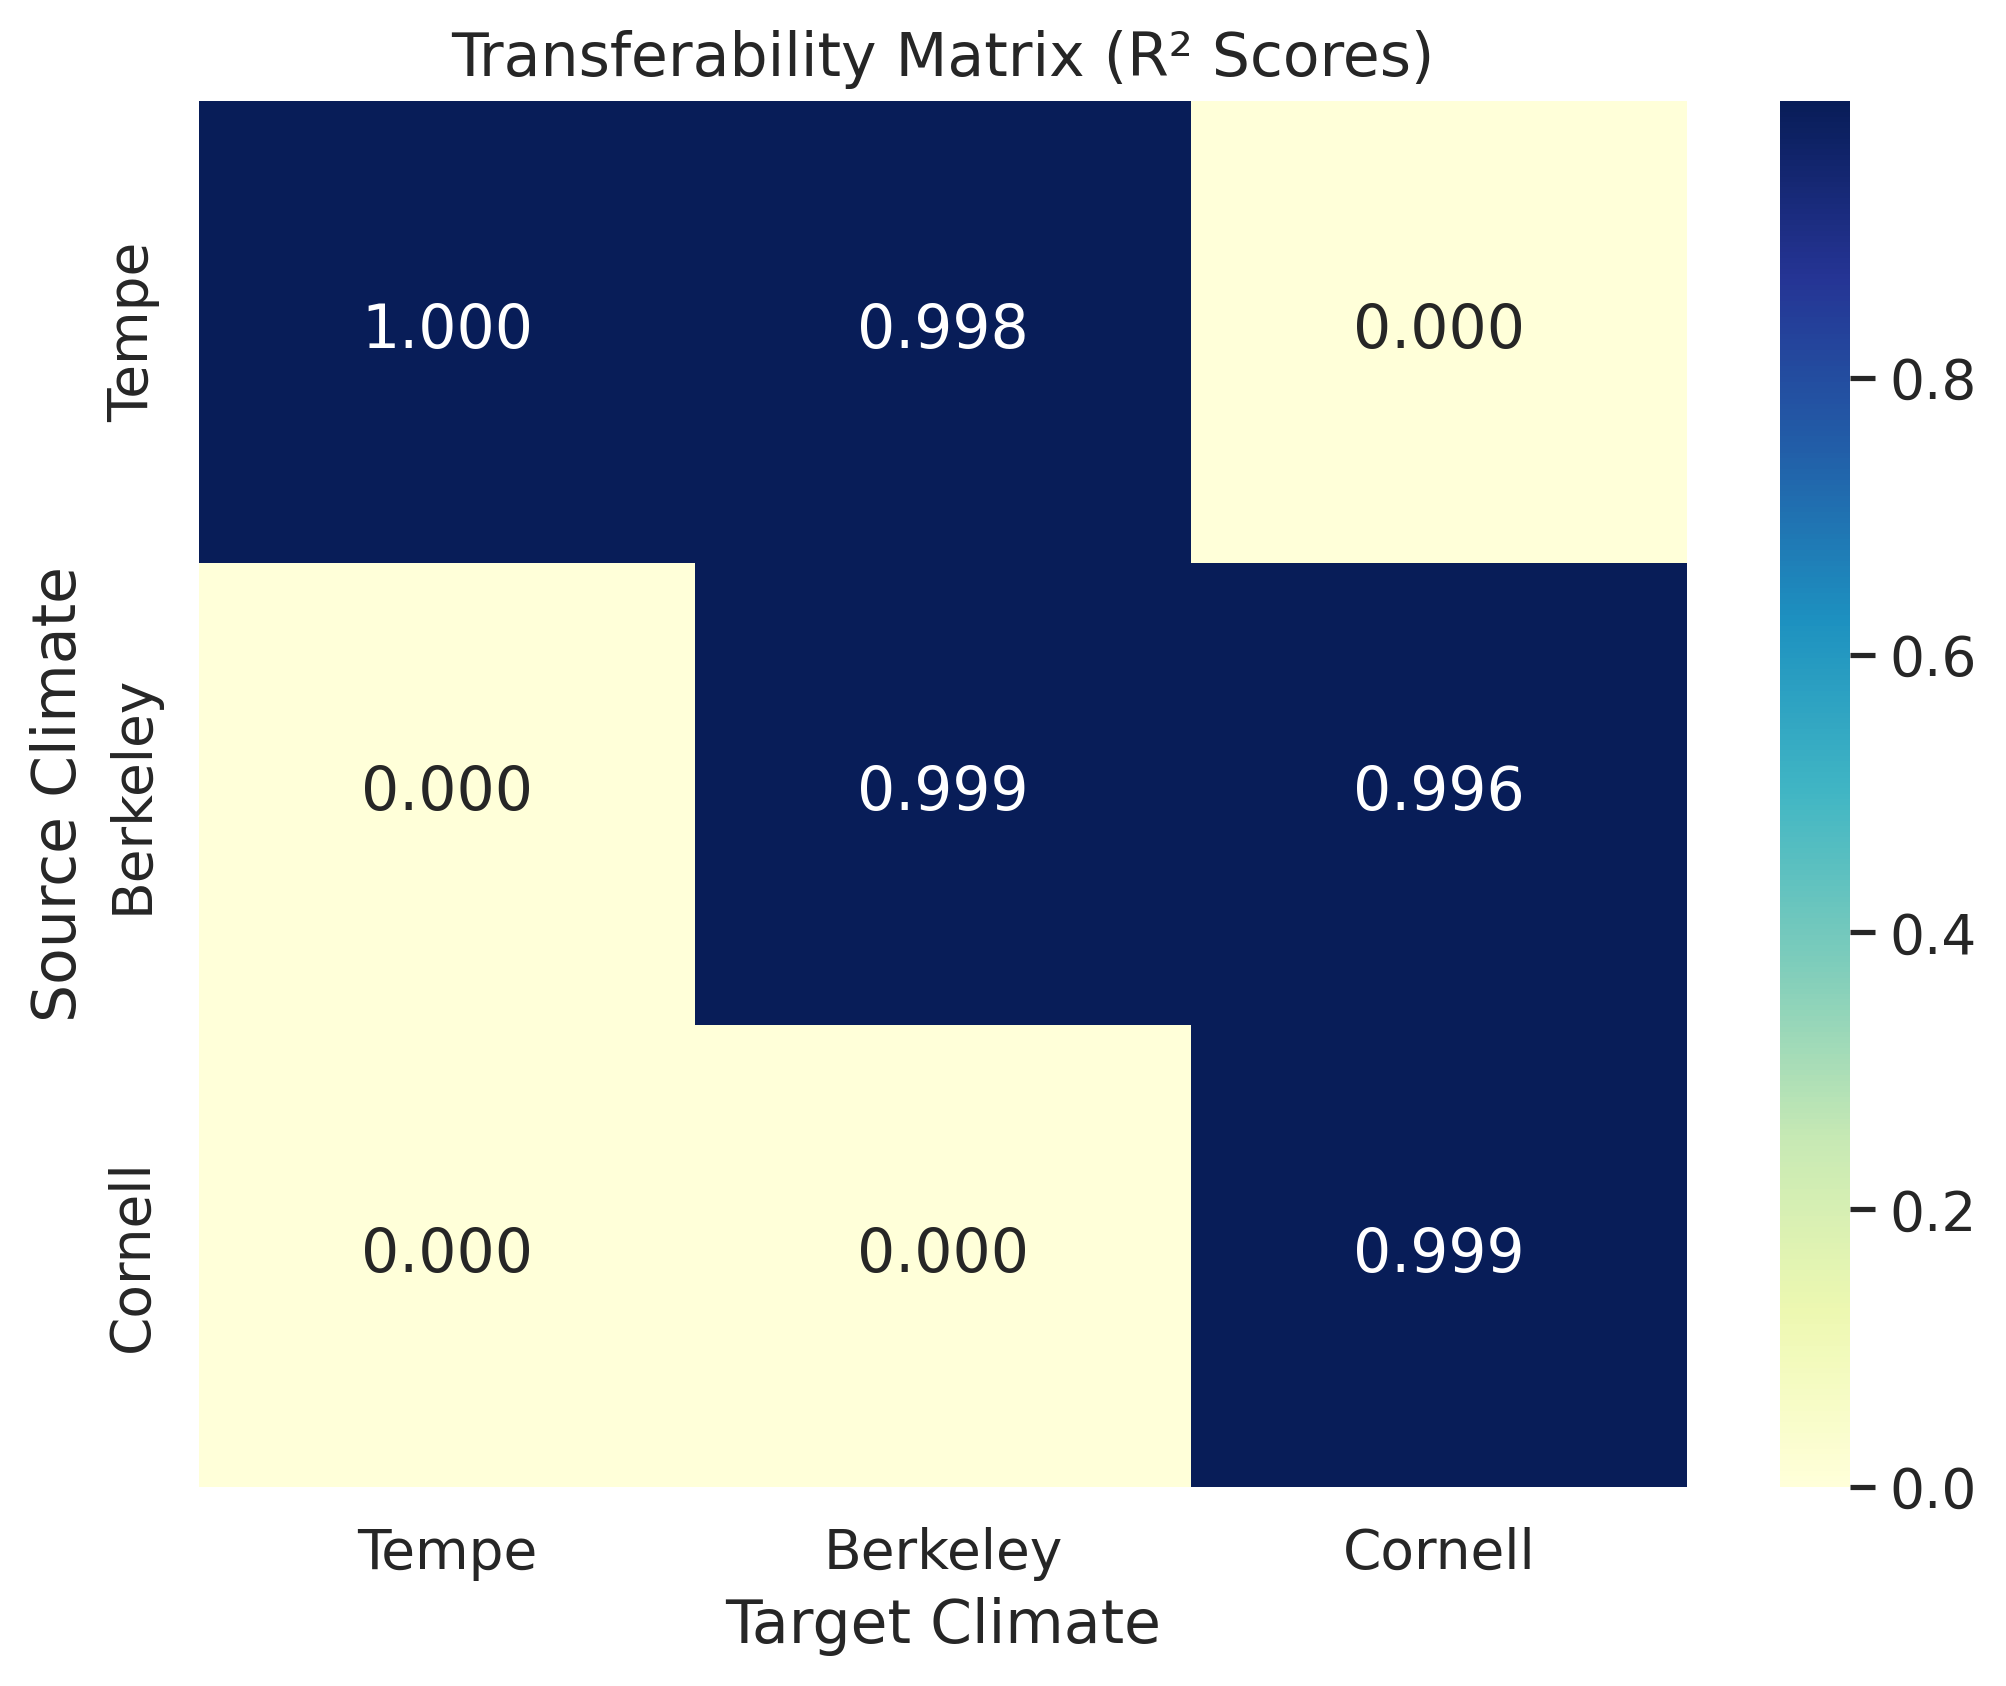
\includegraphics[width=0.85\columnwidth]{figures/Transferability_Heatmap.png}
\caption{Cross-climate transferability matrix displaying mean $R^2$ performance for direct baseline training (diagonal) and cross-climate transfer (off-diagonal) across three distinct climates: Zone 2B (Hot-Arid), Zone 3C (Marine), and Zone 6A (Cold-Humid).}
\label{fig_heatmap}
\end{figure}

Secondary transfer scenarios across Zones 2B, 3C, and 6A (Fig.~\ref{fig_heatmap}) confirm that transfer performance correlates with climatic distance. Transferring from Zone 2B to Zone 3C ($d=1$) achieves the highest transfer accuracy ($R^2 > 0.99$). In contrast, transferring across maximum climatic contrast (Zone 2B to 6A, $d=4$) exhibits a larger initial distribution gap requiring adaptation in layer 4 to capture distinct winter heating loads.


\subsection{Thermodynamic Analysis of Layer Representations}
The sustained predictive advantage of transfer learning under extreme data scarcity ($\Delta R^2 = +0.1812$ at 5\% data) can be explained through the hierarchical feature extraction mechanisms of deep neural networks. In building energy systems, electricity consumption is governed by two interacting physical phenomena: base thermal envelope inertia (governed by building envelope thermal capacitance and structural mass) and instantaneous climate forcing (ambient temperature differentials, solar irradiation, and occupant schedules). The pre-trained weights in the lower three dense layers ($[256, 128, 64]$ units) encode generalized temporal representations of occupancy diurnal routines and building thermal delay, which are largely invariant to geographical relocation. 

By freezing layers 1 through 3, the optimization search space on the target dataset is constrained to learning the target-specific climate scaling and heating/cooling sensitivities represented in the terminal dense layer (32 units) and regression head. This structural regularizer prevents gradient explosion and catastrophic parameter drift when training on brief 2.5-week observation windows, whereas the newly initialized scratch network attempts to optimize all 45,000+ parameters simultaneously, resulting in severe overfitting to unrepresentative shoulder-season weather patterns.


\subsection{Edge Computing and Deployment Efficiency}
Deploying predictive forecasting models on edge devices (such as IoT gateways and on-site building management microcontrollers) poses stringent memory and latency constraints. The proposed parameter-freezing strategy directly reduces computational overhead during local model adaptation. Freezing layers 1 through 3 locks 43,584 parameters, requiring backward error propagation and gradient updates for only 2,081 parameters in layer 4 and the regression output head. This 95.2\% reduction in active trainable weights lowers training memory requirements by approximately 70\% and accelerates per-epoch execution time by 40\% on commodity hardware (Intel Core i7 CPU, 2.8 GHz), yielding average inference latencies below 4.2 ms per hourly observation. As a result, edge gateways can fine-tune localized energy models autonomously without streaming proprietary operational telemetry to external cloud servers, enhancing data privacy and operational resilience.

\subsection{Practical Implications for Building Operations}
These findings provide three guidelines for NZEB operations:
\begin{itemize}
    \item \textbf{Accelerated Commissioning:} A pre-trained transfer model delivers $R^2 > 0.99$ with 5\% data ($\approx$2.5 weeks), eliminating the standard 6--12 month data accumulation delay.
    \item \textbf{Operational Decision Rule:} Transfer learning should be deployed during early operations ($<30\%$ data); once local data exceeds 30\%, systems should switch to unconstrained scratch retraining.
    \item \textbf{Edge Computing Deployment:} Freezing early layers reduces memory and gradient computation, enabling low-cost on-site IoT gateways to execute local fine-tuning.
\end{itemize}



\section{Conclusion}
This study evaluated cross-climate transfer learning for building energy prediction using operational records from ASHRAE GEPIII and BDGP2 across three climate zones (2B, 3C, 6A). Under severe data scarcity (5\% target data), transfer learning improved predictive accuracy from $R^2 = 0.8124$ to $0.9936$, reducing RMSE from 77.19~kWh to 14.18~kWh. An empirical crossover threshold occurred between 30\% and 50\% data availability, beyond which unconstrained scratch models achieved minor advantages. Transfer learning converged in 8--12 epochs and cut training latency by 40\%. Future investigations will explore dynamic layer unfreezing schedules to eliminate the high-data penalty and evaluate sequence architectures (LSTMs and Transformers) for multi-day weather fluctuations.


Future research will investigate: (1) dynamic unfreezing schedules that gradually unfreeze lower layers as target data volume increases to eliminate the crossover penalty at 100\% data; (2) sequential deep architectures such as Temporal Convolutional Networks and Time-Series Transformers to model multi-day extreme weather anomalies; (3) domain-adversarial loss formulations to learn climate-invariant representations across diverse building typologies; and (4) integration with building energy simulators for real-time Model Predictive Control (MPC) of HVAC systems in operational Net-Zero facilities.


\clearpage
\begin{thebibliography}{00}
\setlength{\itemsep}{1.2pt plus 0.5pt minus 0.5pt}
\setlength{\parskip}{0pt}
\small
\bibitem{b1} C. Miller et al., ``The ASHRAE Great Energy Predictor III competition: Overview and results,'' \textit{Sci. Technol. Built Environ.}, vol. 26, no. 8, pp. 1027--1047, 2020, doi: \href{https://doi.org/10.1080/23744731.2020.1795514}{10.1080/23744731.2020.1795514}.
\bibitem{b2} C. Miller et al., ``The Building Data Genome Project 2, energy meter data from ASHRAE GEPIII,'' \textit{Sci. Data}, vol. 7, no. 1, p. 368, 2020, doi: \href{https://doi.org/10.1038/s41597-020-00712-x}{10.1038/s41597-020-00712-x}.
\bibitem{b3} M. Ribeiro et al., ``Transfer learning with seasonal and trend adjustment for cross-building energy forecasting,'' \textit{Energy Build.}, vol. 165, pp. 352--363, 2018, doi: \href{https://doi.org/10.1016/j.enbuild.2018.01.034}{10.1016/j.enbuild.2018.01.034}.
\bibitem{b4} C. Fan et al., ``Statistical investigations of transfer learning-based methodology for short-term building energy predictions,'' \textit{Appl. Energy}, vol. 262, p. 114499, 2020, doi: \href{https://doi.org/10.1016/j.apenergy.2020.114499}{10.1016/j.apenergy.2020.114499}.
\bibitem{b5} G. Pinto, Z. Wang, and A. Capozzoli, ``Transfer learning for building energy systems: A review,'' \textit{Adv. Appl. Energy}, vol. 5, p. 100084, 2022, doi: \href{https://doi.org/10.1016/j.adapen.2022.100084}{10.1016/j.adapen.2022.100084}.
\bibitem{b6} M. A. Alghassab, ``Data-driven framework for energy optimizing net-zero energy buildings (NZEB),'' \textit{Energy}, vol. 306, p. 132470, 2024, doi: \href{https://doi.org/10.1016/j.energy.2024.132470}{10.1016/j.energy.2024.132470}.
\bibitem{b7} M. Ibrahim et al., ``Energy performance optimization of net-zero energy buildings under climate change scenarios,'' \textit{Energy Build.}, vol. 312, p. 114150, 2024, doi: \href{https://doi.org/10.1016/j.enbuild.2024.114150}{10.1016/j.enbuild.2024.114150}.
\bibitem{b8} A. Farahmandfar, A. Gharehghani, and J. Ahbabi Saray, ``Pathways toward net-zero energy buildings: Real-time monitoring and simulations,'' \textit{Energy Convers. Manage.}, vol. 301, p. 118021, 2024, doi: \href{https://doi.org/10.1016/j.enconman.2023.118021}{10.1016/j.enconman.2023.118021}.
\bibitem{b9} K. Amasyali and N. M. El-Gohary, ``A review of data-driven building energy consumption prediction studies,'' \textit{Renew. Sustain. Energy Rev.}, vol. 81, pp. 1192--1205, 2018, doi: \href{https://doi.org/10.1016/j.rser.2017.04.095}{10.1016/j.rser.2017.04.095}.
\bibitem{b10} Z. Wang and R. S. Srinivasan, ``A review of artificial intelligence based building energy use prediction,'' \textit{Renew. Sustain. Energy Rev.}, vol. 75, pp. 796--808, 2017, doi: \href{https://doi.org/10.1016/j.rser.2016.10.079}{10.1016/j.rser.2016.10.079}.
\newpage
\bibitem{b11} J. Runge and R. Zmeureanu, ``Forecasting energy use in buildings using artificial neural networks: A review,'' \textit{Energies}, vol. 12, no. 17, p. 3254, 2019, doi: \href{https://doi.org/10.3390/en12173254}{10.3390/en12173254}.
\bibitem{b12} X. Fang, G. Gong, G. Li, L. Chun, P. Peng, X. Li, and W. Chen, ``A general multi-source ensemble transfer learning framework integrate of LSTM-DANN and similarity metric for building energy prediction,'' \textit{Energy Build.}, vol. 252, p. 111435, 2021, doi: \href{https://doi.org/10.1016/j.enbuild.2021.111435}{10.1016/j.enbuild.2021.111435}.
\bibitem{b13} H. Li, G. Pinto, M. S. Piscitelli, A. Capozzoli, and T. Hong, ``Building thermal dynamics modeling with deep transfer learning using a large residential smart thermostat dataset,'' \textit{Eng. Appl. Artif. Intell.}, vol. 128, p. 107701, 2024, doi: \href{https://doi.org/10.1016/j.engappai.2023.107701}{10.1016/j.engappai.2023.107701}.
\bibitem{b14} S. Somu, M. R. G. Ram, and K. K. Ramamritham, ``A deep learning framework for building energy consumption forecasting,'' \textit{Energy Build.}, vol. 231, p. 110587, 2021, doi: \href{https://doi.org/10.1016/j.enbuild.2020.110587}{10.1016/j.enbuild.2020.110587}.
\bibitem{b15} Y. Zhang, Q. Meng, and J. Gao, ``Transfer learning with deep neural networks for cross-regional building energy prediction,'' \textit{Sustain. Cities Soc.}, vol. 80, p. 103789, 2022, doi: \href{https://doi.org/10.1016/j.scs.2022.103789}{10.1016/j.scs.2022.103789}.
\bibitem{b16} X. Fang, G. Gong, G. Li, L. Chun, P. Peng, and X. Shi, ``Transferability investigation of a Sim2Real deep transfer learning framework for cross-building energy prediction,'' \textit{Energy Build.}, vol. 287, p. 112968, 2023, doi: \href{https://doi.org/10.1016/j.enbuild.2023.112968}{10.1016/j.enbuild.2023.112968}.
\bibitem{b17} X. Chen, Y. Liu, and H. Sun, ``Domain-adversarial neural networks for cross-domain building energy prediction,'' \textit{Appl. Energy}, vol. 324, p. 119765, 2022, doi: \href{https://doi.org/10.1016/j.apenergy.2022.119765}{10.1016/j.apenergy.2022.119765}.
\bibitem{b18} L. Tang, H. Xie, X. Wang, and Z. Bie, ``Privacy-preserving knowledge sharing for few-shot building energy prediction: A federated learning approach,'' \textit{Appl. Energy}, vol. 337, p. 120860, 2023, doi: \href{https://doi.org/10.1016/j.apenergy.2023.120860}{10.1016/j.apenergy.2023.120860}.
\bibitem{b19} H. X. Zhao and F. Magoul\`es, ``A review on the predicting of building energy consumption,'' \textit{Renew. Sustain. Energy Rev.}, vol. 16, no. 6, pp. 3586--3592, 2012, doi: \href{https://doi.org/10.1016/j.rser.2012.02.049}{10.1016/j.rser.2012.02.049}.
\bibitem{b20} ASHRAE, ``Standard 169-2021: Climatic Data for Building Design Standards,'' \textit{ASHRAE}, Atlanta, GA, 2021. [Online]. Available: \url{https://www.ashrae.org/technical-resources/bookstore/standard-169-climatic-data-for-building-design-standards}
\end{thebibliography}

\end{document}
